\chapter{Cài đặt và hiện thực hệ thống}
\label{chap:caidat}

Chương này trình bày cách hiện thực các thành phần đã thiết kế ở Chương~\ref{chap:phantich}. Nội dung đi từ môi trường và tổ chức mã nguồn, qua từng module xử lý, đến các tham số cấu hình cùng cơ sở lựa chọn, cách xử lý lỗi, bảo mật, hiệu năng, triển khai, và cuối cùng là API web cùng giao diện người dùng. Trong chương này, \emph{đoạn} (chunk) là đơn vị lưu trữ và tìm kiếm ứng với một nút của cây Điều--Khoản--Điểm, còn \emph{cạnh trích dẫn} là liên kết từ một đoạn tới đoạn mà nó viện dẫn.

\section{Môi trường và công nghệ}
\label{sec:c4_cong_nghe}

Bảng~\ref{tab:c4_cong_nghe} liệt kê các công nghệ chính, phiên bản được dùng khi đo các kết quả ở Chương~\ref{chap:kiem-thu-danh-gia} và vai trò của từng công nghệ.

\begin{table}[H]
\centering
\caption{Các công nghệ sử dụng, phiên bản và vai trò trong hệ thống}
\label{tab:c4_cong_nghe}
\footnotesize
\renewcommand{\arraystretch}{1.05}
\begin{tabularx}{\textwidth}{@{}>{\raggedright\arraybackslash}p{3.6cm} >{\raggedright\arraybackslash}p{2.6cm} >{\raggedright\arraybackslash}X@{}}
\toprule
\textbf{Công nghệ} & \textbf{Phiên bản} & \textbf{Vai trò} \\
\midrule
Python, \texttt{uv} & 3.13 & Ngôn ngữ của module nạp, bộ tìm kiếm, máy chủ MCP, API web và công cụ đánh giá; \texttt{uv} quản lý thư viện phụ thuộc \\
PostgreSQL & 16.15 & Lưu văn bản, đoạn, chỉ mục từ khoá, cạnh trích dẫn và bộ đệm vector; thực hiện BM25, RRF và tìm kiếm nguyên văn bằng hàm lưu trữ \\
\texttt{pgvector} & 0.8.6 & Kiểu vector, độ đo cosine và chỉ mục HNSW \cite{malkov2020hnsw} \\
\texttt{ltree}, \texttt{unaccent} & đi kèm PostgreSQL & Đường dẫn phân cấp và lọc theo nhánh cây; bỏ dấu tiếng Việt \\
Sentence Transformers, PyTorch & 6.0.1; 2.13.0 & Chạy Qwen3-Embedding-0.6B \cite{zhang2025qwen3} để mã hoá câu hỏi và đoạn \\
FastAPI, Pydantic, Uvicorn & 0.141; 2.13; 0.52 & API web và kiểm tra dữ liệu vào ra \\
\texttt{asyncpg} & 0.31.0 & Kết nối bất đồng bộ tới cơ sở dữ liệu \\
MCP SDK & 2.1.1 & Máy chủ Model Context Protocol \cite{anthropic2024mcp} \\
React, Vite, TypeScript, Tailwind CSS & 18.3; 6.1; 5.7; 3.4 & Giao diện trang đơn \\
Claude Code, Codex, Antigravity & bản cài đặt tại thời điểm đo & Chương trình dòng lệnh gọi mô hình ngôn ngữ lớn để trả lời (Mục~\ref{sec:cd-agent}) \\
Docker Compose & -- & Khởi chạy PostgreSQL kèm \texttt{pgvector} \\
\bottomrule
\end{tabularx}
\end{table}

Quá trình phát triển dùng thêm \texttt{ruff} và \texttt{ty} để kiểm tra phong cách mã và kiểu tĩnh, Playwright để tự động hoá trình duyệt khi kiểm thử giao diện, và Git cùng GitHub để quản lý mã nguồn theo nhánh. Phép đo độ trễ được thực hiện trên CPU Intel Xeon W-10855M (6 nhân, 32 GB RAM); việc mã hoá toàn bộ kho văn bản dùng GPU có 4 GB bộ nhớ.

Các công nghệ được lựa chọn theo ba tiêu chí. Thứ nhất, toàn bộ dữ liệu phục vụ tìm kiếm nằm trong một cơ sở dữ liệu duy nhất, nhờ đó cả ba nhánh tìm kiếm cùng lọc theo ngày vi phạm và phạm vi văn bản trong một câu truy vấn. Thứ hai, mô hình embedding chạy cục bộ trên phần cứng phổ thông, không phụ thuộc dịch vụ bên ngoài khi tìm kiếm. Thứ ba, bộ công cụ tra cứu được tách khỏi mô hình sinh qua một giao thức chuẩn, nên có thể thay chương trình trả lời mà không phải sửa phần tra cứu.

\section{Tổ chức mã nguồn}
\label{sec:cd-macnguon}

Mã nguồn được chia thành các gói tương ứng với bốn tầng của kiến trúc ở Hình~\ref{fig:kientruc}. Bảng~\ref{tab:cd-goi} trình bày ánh xạ giữa gói, tầng kiến trúc và chức năng.

\begin{table}[H]
\centering
\caption{Ánh xạ các gói mã nguồn vào kiến trúc bốn tầng}
\label{tab:cd-goi}
\footnotesize
\begin{tabularx}{\textwidth}{@{}l l X@{}}
\toprule
\textbf{Gói} & \textbf{Tầng} & \textbf{Chức năng} \\
\midrule
\texttt{ingestion} & (1) Nạp văn bản & Trích xuất tệp Word, xử lý ngoặc kép, phân tích cây, tạo đoạn, liên kết trích dẫn, tính vector \\
\texttt{db} & (2) Lưu trữ & Kết nối, 22 tệp migration lược đồ, hàm lưu trữ, xuất và nhập bản chụp dữ liệu \\
\texttt{retrieval} & (3) Tra cứu & Chỉ mục văn bản sửa đổi, bộ xếp hạng lại \\
\texttt{mcp} & (3) Tra cứu & Máy chủ MCP và các công cụ tra cứu, bảo trì đồ thị \\
\texttt{answer} & (4) Trả lời & Gọi chương trình trả lời, chế độ agent, kiểm tra bám nguồn \\
\texttt{web}, \texttt{frontend} & (4) Giao diện & API web và ứng dụng giao diện \\
\texttt{eval} & (4) Đánh giá & Chạy bộ đánh giá tìm kiếm và câu trả lời trên cùng đường xử lý của sản phẩm \\
\bottomrule
\end{tabularx}
\end{table}

Mọi thao tác vận hành, từ nạp văn bản, tính vector, chạy đánh giá đến khởi động máy chủ, đều đi qua một giao diện dòng lệnh duy nhất. Cách tổ chức này bảo đảm số liệu ở Chương~\ref{chap:kiem-thu-danh-gia} được đo trên đúng mã nguồn mà người dùng sử dụng.

\section{Module nạp văn bản}
\label{sec:cd-napvanban}

\subsection{Trích xuất văn bản nguồn}

Bước trích xuất chuyển tệp Word gốc thành văn bản chuẩn theo dòng; số dòng của văn bản chuẩn là hệ toạ độ chung cho mọi thành phần phía sau. Bước này xử lý ba đặc điểm định dạng thường gặp trong văn bản hành chính.

\begin{itemize}
    \item \textbf{Đánh số tự động.} Nhiều văn bản dùng tính năng đánh số tự động của Word cho Khoản và Điểm, nên nhãn ``1.'' hay ``a)'' không nằm trong nội dung chữ. Hệ thống khôi phục các nhãn này bằng một bộ đếm riêng cho từng cấp thụt lề.
    \item \textbf{Bảng dàn trang.} Quốc hiệu, tiêu ngữ và chữ ký thường được đặt trong bảng ẩn đường viền. Một bảng chỉ được giữ ở dạng bảng khi có khung viền bao quanh, có tối thiểu hai hàng dữ liệu và ít nhất 40\% số ô chứa nội dung; các bảng còn lại được chuyển thành văn bản thường. Ngưỡng được đặt nghiêng về phía văn bản thường vì hai loại sai có hậu quả không cân xứng: một bảng thật bị coi là văn bản vẫn giữ nguyên nội dung, còn một đoạn văn bị coi là bảng sẽ bị cắt thành các ô và mất mạch câu.
    \item \textbf{Mục lục.} Phần mục lục ở đầu một số văn bản được nhận diện và loại bỏ để không bị phân tích nhầm thành Điều.
\end{itemize}

Sau khi trích xuất, hệ thống kiểm tra rằng mọi phần tử chữ trong tệp gốc đều có mặt trong văn bản chuẩn. Một văn bản không qua được bước kiểm tra này bị từ chối nạp, thay vì được nạp với nội dung bị thiếu.

\subsection{Phân tích cấu trúc}

Trong văn bản sửa đổi, lời văn mới của điều khoản được đặt trong ngoặc kép ngay sau câu lệnh sửa đổi; chẳng hạn câu ``a) Sửa đổi, bổ sung điểm đ như sau:'' được theo sau bởi dòng ``đ)'' nằm trong ngoặc kép. Vì vậy, trước khi phân tích, hệ thống xác định mọi khoảng nằm trong ngoặc kép, kể cả trường hợp văn bản gốc thiếu dấu đóng ngoặc ở cuối dòng, và coi nội dung trong đó là văn bản thường. Bộ phân tích sau đó dựng cây theo các bước sau.

\begin{enumerate}
    \item Duyệt văn bản chuẩn theo từng dòng, giữ một ngăn xếp các nút đang mở, từ văn bản gốc xuống tới cấp sâu nhất.
    \item Với mỗi dòng nằm ngoài ngoặc kép, nhận diện ký hiệu đề mục ở đầu dòng (Phần, Chương, Mục, Điều, Khoản, Điểm) theo quy ước đánh số của từng cấp.
    \item Chỉ công nhận một ký hiệu là nút mới khi nó là số kế tiếp của nút cùng cấp đang mở, hoặc là số 1 mở đầu một cấp con. Quy tắc này ngăn việc nhận nhầm một số tiền đứng đầu dòng, chẳng hạn ``7.500 đồng'', thành Khoản 500 của Điều 7.
    \item Khi một nút mới được công nhận, đóng các nút cùng cấp hoặc sâu hơn trên ngăn xếp, rồi đặt nút mới làm con của nút đang mở gần nhất. Dòng không có ký hiệu đề mục được gán cho nút đang mở.
    \item Khi gặp phần nơi nhận hoặc chức danh người ký, ngừng nhận diện điều khoản; nếu phía sau có quy chế, quy định hoặc quy chuẩn ban hành kèm theo, mở một nút văn bản đính kèm và tiếp tục phân tích theo Điều--Khoản.
\end{enumerate}

Hai trường hợp đặc biệt cần xử lý riêng. Với các phụ lục và quy chuẩn không chia theo Điều--Khoản, như QCVN 41:2024/BGTVT, bộ phân tích nhận diện ba tầng đề mục là chữ cái, số La Mã và số thập phân, đồng thời dùng thứ tự bảng chữ cái để phân biệt chữ ``I'' đứng sau mục ``H'' với số La Mã ``I''. Ngoài ra, theo quy ước soạn thảo, các Điểm kết thúc bằng dấu chấm phẩy và Điểm cuối cùng kết thúc bằng dấu chấm; một dòng viết hoa nằm sau Điểm đã kết thúc bằng dấu chấm vì vậy được xem là đoạn kết của Khoản, trừ khi phía sau lại xuất hiện thêm một Điểm kế tiếp.

\subsection{Tạo đoạn}

Bộ tạo đoạn duyệt cây theo chiều sâu: nút lá nhận toàn bộ phạm vi dòng của nó, còn nút có con chỉ nhận phần văn bản dẫn nhập đứng trước nút con đầu tiên. Mỗi đoạn được lưu ở hai dạng: nguyên văn để hiển thị, và văn bản kèm ngữ cảnh để tính vector và lập chỉ mục từ khoá. Văn bản kèm ngữ cảnh được ghép từ tên văn bản, nhãn Chương, tên Điều, câu dẫn khung phạt của Khoản và nguyên văn của đoạn. Bảng~\ref{tab:cd-vidu-doan} minh hoạ hai dạng này với Điểm c Khoản 7 Điều 7 Nghị định 168/2024/NĐ-CP: riêng nguyên văn không cho biết hành vi thuộc loại xe nào và bị phạt bao nhiêu, trong khi văn bản kèm ngữ cảnh chứa đủ cả hai thông tin.

\begin{table}[H]
\centering
\caption{Nguyên văn và văn bản kèm ngữ cảnh của Điểm c Khoản 7 Điều 7 Nghị định 168/2024/NĐ-CP}
\label{tab:cd-vidu-doan}
\footnotesize
\begin{tabularx}{\textwidth}{@{}>{\raggedright\arraybackslash}p{2.6cm} >{\raggedright\arraybackslash}X@{}}
\toprule
\textbf{Dạng} & \textbf{Nội dung} \\
\midrule
Nguyên văn & c) Không chấp hành hiệu lệnh của đèn tín hiệu giao thông; \\
Kèm ngữ cảnh & [Nghị định quy định xử phạt vi phạm hành chính về trật tự, an toàn giao thông trong lĩnh vực giao thông đường bộ; trừ điểm, phục hồi điểm giấy phép lái xe] > [Chương II] > [Điều 7: Xử phạt, trừ điểm giấy phép lái của người điều khiển xe mô tô, xe gắn máy, các loại xe tương tự xe mô tô và các loại xe tương tự xe gắn máy vi phạm quy tắc giao thông đường bộ] > [Khoản 7: Phạt tiền từ 4.000.000 đồng đến 6.000.000 đồng đối với người điều khiển xe thực hiện một trong các hành vi vi phạm sau đây] \newline c) Không chấp hành hiệu lệnh của đèn tín hiệu giao thông; \\
\bottomrule
\end{tabularx}
\end{table}

Tiêu đề Chương chỉ được giữ ở dạng nhãn ngắn để không lặp lại ở hàng trăm đoạn, trong khi tiêu đề Phụ lục được giữ nguyên vì thường chứa tên nhóm biển báo hoặc tên bảng kỹ thuật. Văn bản kèm ngữ cảnh của mỗi đoạn được giới hạn ở 25.000 ký tự, kể cả phần ngữ cảnh; đoạn nào vượt giới hạn được chia theo ranh giới dòng thành nhiều cửa sổ, mỗi cửa sổ lặp lại tên bảng, đơn vị tính và dòng tiêu đề cột. Với kho hiện tại, chỉ 4 trong 6.775 đoạn phải chia cửa sổ, và đoạn dài nhất có 24.915 ký tự. Cuối cùng, hệ thống kiểm tra điều kiện phủ dòng: mỗi dòng có nội dung, trừ dòng tiêu đề và biểu mẫu, phải thuộc về đúng một đoạn; nếu không, quá trình nạp dừng lại và báo số dòng bị thiếu hoặc bị trùng.

\subsection{Liên kết trích dẫn}

Bộ liên kết chỉ tạo cạnh cho các cụm trích dẫn nội bộ nằm ngoài ngoặc kép và được neo bởi từ ``này'', như ``điểm a khoản 9 Điều này''. Các trích dẫn sang văn bản khác không được tạo tự động, vì việc xác định chính xác văn bản đích đòi hỏi kiểm chứng thêm (Mục~\ref{sec:cd-mcp}). Bảng~\ref{tab:cd-tridan} tóm tắt các hiện tượng ngôn ngữ mà bộ liên kết xử lý.

\begin{table}[H]
\centering
\caption{Các hiện tượng trích dẫn nội bộ và cách xử lý}
\label{tab:cd-tridan}
\footnotesize
\begin{tabularx}{\textwidth}{@{}>{\raggedright\arraybackslash}p{3.2cm} >{\raggedright\arraybackslash}p{4.2cm} >{\raggedright\arraybackslash}X@{}}
\toprule
\textbf{Hiện tượng} & \textbf{Ví dụ} & \textbf{Cách xử lý} \\
\midrule
Văn bản đính kèm & ``Điều 5 Quy chế này'' & Xác định phạm vi theo loại văn bản đứng trước từ ``này'' \\
Danh sách viết gộp & ``điểm a, điểm b khoản 6 Điều này'' & Các mục đứng trước dùng chung Khoản, Điều nêu ở cuối cụm \\
Dạng thu hẹp & ``Điều 20 (điểm c khoản 3)'' & Chỉ trỏ tới Điểm c Khoản 3 Điều 20 \\
Khoảng liên tiếp & ``từ khoản 1 đến khoản 3'' & Mở rộng theo thứ tự thực tế trên cây, kể cả khoản chèn thêm như Khoản 2a \\
Cụm có nhiều cách hiểu & ``điểm a, b khoản 1, 2'' & Bỏ qua, không tạo cạnh \\
Đích ở cấp Điều, Khoản & ``khoản 2 Điều này'' & Mở rộng xuống mọi đoạn lá bên dưới \\
\bottomrule
\end{tabularx}
\end{table}

Kết quả trên kho hiện tại là 10.570 cạnh trích dẫn. Mỗi cạnh lưu kèm cụm từ trích dẫn nguyên văn, nên luôn có thể kiểm tra lại cạnh đó bằng cách đối chiếu với văn bản nguồn.

\section{Module tìm kiếm}
\label{sec:cd-timkiem}

\subsection{Biểu diễn vector}

Các đoạn được mã hoá bằng Qwen3-Embedding-0.6B. Vector đầu ra 1.024 chiều được cắt còn 512 chiều theo phương pháp Matryoshka \cite{kusupati2022mrl} rồi chuẩn hoá L2. Khi mã hoá câu hỏi, hệ thống dùng lời nhắc truy vấn do mô hình định nghĩa, còn các đoạn được mã hoá không kèm lời nhắc; Chương~\ref{chap:kiem-thu-danh-gia} cho thấy lời nhắc này cải thiện Hit@1 có ý nghĩa thống kê. Mô hình chạy ở độ chính xác FP16 trên GPU và FP32 trên CPU; khi mã hoá cả kho, các đoạn được xử lý theo lô 32, sắp từ dài đến ngắn, và kích thước lô tự giảm một nửa khi GPU hết bộ nhớ. Vì mô hình nhận tối đa 32.768 token, giới hạn 25.000 ký tự của mỗi đoạn bảo đảm không đoạn nào bị cắt khi mã hoá. Vector đã tính được lưu trong bộ đệm theo mã băm của văn bản, nên khi nạp lại một văn bản, chỉ những đoạn có nội dung thay đổi mới phải tính lại.

\subsection{Chỉ mục từ khoá}

Trước khi lập chỉ mục, các ký hiệu số chú thích dính liền vào chữ trong văn bản hợp nhất được tách ra. Văn bản kèm ngữ cảnh của mỗi đoạn được bỏ dấu, chuyển về chữ thường và tách thành âm tiết. Chỉ mục ngược lưu cả âm tiết đơn lẫn cặp hai âm tiết liền kề cùng tần suất xuất hiện, tổng cộng 995.937 bản ghi trên kho hiện tại, và được trigger cập nhật tự động mỗi khi một đoạn thay đổi.

\subsection{Quy trình tìm kiếm lai}

Toàn bộ quy trình tìm kiếm lai được thực hiện trong một hàm lưu trữ của PostgreSQL theo các bước sau, với $n$ là số kết quả cần trả về.

\begin{enumerate}
    \item Tính số đoạn $N$ và độ dài trung bình của các đoạn, là hai đại lượng dùng trong công thức BM25.
    \item Nhánh vector: lấy $\max(6n, 120)$ đoạn có khoảng cách cosine nhỏ nhất tới vector câu hỏi, chỉ trong các đoạn còn hiệu lực vào ngày vi phạm và thuộc phạm vi văn bản, nhánh cây đã chọn.
    \item Nhánh từ khoá: tách câu truy vấn thành âm tiết và cặp âm tiết, đọc các bản ghi tương ứng trong chỉ mục ngược, tính điểm BM25 \cite{robertson2009bm25} với $k_1 = 1{,}2$ và $b = 0{,}75$, rồi lấy $\max(6n, 120)$ đoạn có điểm cao nhất với cùng các điều kiện lọc.
    \item Hợp nhất hai danh sách bằng RRF \cite{cormack2009rrf} với $k = 20$; một đoạn chỉ xuất hiện ở một nhánh vẫn nhận điểm từ nhánh đó.
    \item Trả về $n$ đoạn có điểm RRF cao nhất, kèm độ tương đồng cosine và dấu hiệu cho biết đoạn có khớp ít nhất một cặp âm tiết của câu truy vấn hay không.
\end{enumerate}

Vì các điều kiện lọc được áp dụng ngay trong từng nhánh, hai nhánh luôn chọn ứng viên trên cùng một tập đoạn hợp lệ. Ở quy mô hiện tại, bộ lập kế hoạch truy vấn của PostgreSQL chọn quét tuần tự toàn bộ 6.775 đoạn rồi sắp xếp theo khoảng cách, thay vì dùng chỉ mục HNSW. Nhánh vector vì vậy là tìm kiếm chính xác: phép đo trên 715 câu của bộ đánh giá cho thấy 120 ứng viên của nhánh vector trùng hoàn toàn với kết quả tìm kiếm vét cạn. Chỉ mục HNSW chỉ được dùng khi kho lớn hơn nhiều; khi đó cần đo lại độ phủ vì việc kết hợp chỉ mục xấp xỉ với điều kiện lọc có thể làm thiếu ứng viên.

Khi câu truy vấn được gõ hoàn toàn không dấu, nhánh vector bị tắt và chỉ nhánh từ khoá được dùng. Lý do là kho văn bản được mã hoá từ chữ có dấu, nên vector của câu không dấu thường nằm xa đáp án, trong khi chỉ mục từ khoá đã bỏ dấu vẫn khớp chính xác. Hệ thống không khôi phục dấu cho câu truy vấn vì việc khôi phục dấu tự động có thể sai nghĩa và tạo thêm một nguồn lỗi khó kiểm soát.

\subsection{Công cụ tìm kiếm kết hợp}

Công cụ tìm kiếm cung cấp cho agent kết hợp tìm kiếm lai với tìm kiếm nguyên văn. Hai bước được thực hiện lần lượt: trước hết là tìm kiếm lai theo câu truy vấn, sau đó là tìm các đoạn chứa cụm từ (hoặc biểu thức chính quy) do agent chỉ định. Các kết quả của tìm kiếm nguyên văn được xếp theo độ tương đồng cosine với câu truy vấn thay vì theo thứ tự xuất hiện trong văn bản; nhờ vậy, khi một cụm từ phổ biến như ``phục hồi điểm'' khớp hàng trăm đoạn, những đoạn gần nghĩa nhất với câu hỏi vẫn được đưa lên đầu.

Kết quả cuối được xếp thành ba nhóm theo thứ tự ưu tiên. Nhóm thứ nhất gồm các kết quả của tìm kiếm lai có chứa cụm từ chỉ định, tức là được cả hai cách tìm xác nhận. Nhóm thứ hai gồm các kết quả của tìm kiếm lai không chứa cụm từ đó. Nhóm thứ ba gồm các kết quả chỉ tìm thấy nhờ tìm kiếm nguyên văn. Các điều khoản cùng ngữ cảnh cha được gom lại để không lặp lại phần tiêu đề và câu dẫn.

\subsection{Mức độ tin cậy và bộ xếp hạng lại}

Mỗi kết quả tìm kiếm được gắn một trong ba mức độ tin cậy. Mức ``không có'' được gán khi không đoạn nào khớp ít nhất một cặp âm tiết của câu truy vấn; ở chế độ trả lời một lần, mức này khiến hệ thống từ chối trả lời mà không gọi mô hình ngôn ngữ. Trên 715 câu của bộ đánh giá, không câu nào bị gán mức này, nghĩa là điều kiện từ chối không chặn nhầm câu hỏi trong phạm vi. Mức ``thấp'' được gán khi độ tương đồng cosine cao nhất nhỏ hơn 0,86 và chỉ dùng để hiển thị cảnh báo trên giao diện; câu truy vấn không dấu luôn được xếp mức ``cao'' khi đã khớp từ khoá, vì khi đó độ tương đồng vector không còn ý nghĩa.

Ngưỡng 0,86 được đặt từ phiên bản mô hình embedding trước và chưa được hiệu chỉnh lại sau khi chuyển sang Qwen3-Embedding 512 chiều. Phép đo trên 715 câu cho thấy độ tương đồng cao nhất có trung vị 0,775, phân vị thứ 5 là 0,632, và 652 câu (91\%) bị xếp mức ``thấp'' dù đều thuộc phạm vi. Vì mức ``thấp'' không ảnh hưởng tới kết quả tìm kiếm hay câu trả lời, sai lệch này không làm thay đổi các số liệu ở Chương~\ref{chap:kiem-thu-danh-gia}, nhưng làm cảnh báo trên giao diện mất giá trị thông tin. Ngưỡng cần được hiệu chỉnh lại theo phân bố đo được, chẳng hạn đặt ở phân vị thứ 5 của các câu trong phạm vi.

Mã nguồn còn có một bộ xếp hạng lại dạng cross-encoder đa ngôn ngữ (mMiniLMv2 huấn luyện trên mMARCO), chấm lại 10 kết quả đầu với độ dài tối đa 256 token. Bộ xếp hạng lại mặc định tắt và không được bật trong bất kỳ cấu hình nào ở Chương~\ref{chap:kiem-thu-danh-gia}; tác động của nó chưa được đánh giá và được xếp vào hướng phát triển.

\section{Module ghi chú văn bản sửa đổi}
\label{sec:cd-suadoi}

Bộ suy diễn sửa đổi xây dựng một chỉ mục các điều khoản bị sửa đổi theo các bước sau.

\begin{enumerate}
    \item Với mỗi văn bản sửa đổi, che toàn bộ nội dung nằm trong ngoặc kép để lời văn mới không bị hiểu nhầm là câu lệnh.
    \item Thu thập các câu mở đầu bằng động từ sửa đổi như ``sửa đổi'', ``bổ sung'', ``bãi bỏ'', ``thay thế'' hoặc ``bỏ''.
    \item Với mỗi câu lệnh, tìm câu lệnh bao ngoài gần nhất và kế thừa từ đó văn bản đích, Điều và Khoản; câu lệnh ở cấp cao nhất lấy văn bản đích từ tên văn bản được nêu trong câu.
    \item Đọc các địa chỉ điều khoản trong câu lệnh, bổ sung các cấp còn thiếu từ phạm vi kế thừa, rồi mở rộng thành danh sách các đoạn cụ thể trên cây của văn bản đích.
    \item Chỉ những câu lệnh không bao câu lệnh nào khác mới sinh ra ghi chú; câu lệnh cấp cha chỉ truyền phạm vi xuống dưới, nhờ đó khi văn bản mới chỉ sửa một Điểm, ghi chú không bị gắn lên toàn bộ Điều.
\end{enumerate}

Ba quy tắc bổ sung giúp giải đúng các dạng câu lệnh phức tạp. Với dạng ``Sửa đổi, bổ sung một số cụm từ tại khoản 2 Điều 5 bằng cụm từ\ldots'', bộ suy diễn chỉ lấy điều khoản đích đứng sau giới từ ``tại'' và bỏ qua phần đứng sau ``bằng'', để không nhận nhầm số hiệu văn bản trong cụm từ thay thế thành văn bản bị sửa đổi. Với dạng ``Bổ sung điểm d vào sau điểm c khoản 2 Điều 10'', bộ suy diễn tách điều khoản mới khỏi mốc vị trí, rồi lấy Khoản và Điều từ mốc vị trí để xác định đầy đủ địa chỉ của điểm được bổ sung. Với dạng ``Sửa đổi tên Điều 6'', ghi chú chỉ được gắn vào tiêu đề và phần thân trực tiếp của Điều, không lan xuống các Khoản và Điểm.

Trên kho hiện tại, bộ suy diễn xác định 109 câu lệnh sửa đổi với 183 địa chỉ đích và gắn ghi chú cho 366 đoạn. Khi trả kết quả tìm kiếm, ghi chú chỉ được gắn nếu câu lệnh sửa đổi đã có hiệu lực tại ngày vi phạm được xét; mỗi ghi chú cho biết văn bản sửa đổi, câu lệnh sửa đổi và ngày áp dụng.

\section{Máy chủ MCP và bảo trì đồ thị trích dẫn}
\label{sec:cd-mcp}

Máy chủ MCP giao tiếp với client qua luồng vào ra chuẩn. Khi khởi động, máy chủ đọc danh mục văn bản cùng thời hạn hiệu lực từ cơ sở dữ liệu và đưa vào phần chỉ dẫn gửi cho agent, nhờ đó agent biết chính xác các văn bản đang có trong kho. Máy chủ cung cấp năm công cụ (Bảng~\ref{tab:mcp-tools}); mọi kết quả đều kèm số hiệu văn bản, đường dẫn phân cấp và phạm vi dòng để có thể đối chiếu với văn bản gốc.

\begin{table}[H]
\centering
\caption{Các công cụ của máy chủ MCP}
\label{tab:mcp-tools}
\footnotesize
\begin{tabularx}{\textwidth}{@{}l >{\raggedright\arraybackslash}X@{}}
\toprule
\textbf{Công cụ} & \textbf{Chức năng} \\
\midrule
\texttt{search} & Tìm kiếm lai kết hợp tìm kiếm nguyên văn (Mục~\ref{sec:cd-timkiem}); lọc được theo ngày vi phạm, danh sách văn bản và nhánh cây; kết quả kèm nhóm ưu tiên và ghi chú sửa đổi \\
\texttt{hierarchical\_navigate} & Đọc các đoạn thuộc một nhánh cây, hoặc mở rộng lên Khoản cha để lấy câu dẫn khung phạt, theo đúng thứ tự trong văn bản; tối đa 100 đoạn mỗi lần gọi \\
\texttt{graph\_traverse} & Đi theo các cạnh trích dẫn từ một điều khoản; mặc định theo chiều đi, có thể chọn chiều đến hoặc cả hai chiều, độ sâu từ 1 đến 4 \\
\texttt{get\_raw} & Đọc tối đa 100 dòng liên tiếp của văn bản chuẩn theo số dòng \\
\texttt{graph\_curate\_edges} & Công cụ bảo trì: thêm hoặc gỡ cạnh trích dẫn trong một giao dịch, có kiểm chứng nguyên văn; không được cấp cho agent trả lời \\
\bottomrule
\end{tabularx}
\end{table}

Khi đọc theo nhánh cây, các đoạn chỉ được gộp khi liền kề nhau và có cùng ngữ cảnh cha, nhờ đó đoạn kết của một Khoản không bị đẩy lên trước các Điểm. Khi duyệt đồ thị, công cụ ghi nhớ các đỉnh đã thăm để tránh vòng lặp khi hai điều khoản trích dẫn lẫn nhau. Các giới hạn 100 đoạn, 100 dòng và độ sâu 4 nhằm giữ kích thước mỗi kết quả trong khả năng đọc của agent: Điều dài nhất trong kho có 113 đoạn, nên với những Điều như vậy agent đọc theo từng Khoản; còn duyệt đồ thị quá 4 bước làm số điều khoản tăng nhanh mà ít khi còn liên quan tới câu hỏi.

Công cụ thứ năm phục vụ việc bảo trì đồ thị trích dẫn, chủ yếu để bổ sung các trích dẫn liên văn bản mà bộ liên kết lúc nạp không xử lý, chẳng hạn một điều khoản của Nghị định 168/2024/NĐ-CP dẫn tới quy tắc trong Luật Trật tự, an toàn giao thông đường bộ. Mỗi cạnh mới phải kèm cụm từ trích dẫn xuất hiện nguyên văn trong điều khoản nguồn; nếu cụm từ không có trong nguồn hoặc cạnh trỏ về chính nó, toàn bộ giao dịch bị huỷ. Mọi thay đổi được ghi vào nhật ký cùng lý do, và khi văn bản được nạp lại, các cạnh vẫn thoả điều kiện kiểm chứng được giữ nguyên.

\section{Module trả lời}
\label{sec:cd-agent}

\subsection{Các chương trình trả lời}

Hệ thống gọi mô hình ngôn ngữ lớn thông qua các chương trình dòng lệnh đã được cài đặt và đăng nhập trên máy chủ, thay vì gọi trực tiếp API của nhà cung cấp. Bảng~\ref{tab:cd-providers} liệt kê các chương trình được hỗ trợ; danh sách những chương trình có sẵn trên máy được trả về qua API để giao diện hiển thị.

\begin{table}[H]
\centering
\caption{Các chương trình trả lời được hỗ trợ}
\label{tab:cd-providers}
\footnotesize
\begin{tabularx}{\textwidth}{@{}l l l X@{}}
\toprule
\textbf{Chương trình} & \textbf{Trả lời một lần} & \textbf{Chế độ agent} & \textbf{Ghi chú} \\
\midrule
Claude Code & Có & Có & Cấu hình dùng cho mọi phép đo ở Chương~\ref{chap:kiem-thu-danh-gia} \\
Codex & Có & Không & Chỉ định mô hình mà tài khoản đăng nhập được phép dùng \\
Antigravity & Có & Có & Chế độ agent cần cấp quyền trước cho bốn công cụ chỉ đọc \\
\bottomrule
\end{tabularx}
\end{table}

\subsection{Chế độ agent}

Ở chế độ agent, hệ thống khởi chạy chương trình trả lời ở chế độ không tương tác trong một thư mục tạm rỗng, với cấu hình chỉ gồm máy chủ MCP của hệ thống và danh sách công cụ được phép chỉ gồm bốn công cụ chỉ đọc. Mỗi câu hỏi có thời hạn 300 giây; với Claude Code, số lượt hội thoại của agent còn được giới hạn ở 10, trong đó một lượt có thể gồm nhiều lần gọi công cụ. Lời nhắc yêu cầu agent chỉ dùng thông tin từ công cụ, diễn đạt lại câu hỏi bằng thuật ngữ văn bản luật trước khi tìm kiếm, mở rộng lên Khoản cha để lấy mức phạt, đi theo trích dẫn và đọc điều khoản sửa đổi khi cần, rồi kết thúc bằng câu trả lời có đánh số trích dẫn cùng danh sách đường dẫn của các điều khoản nguồn.

Kết quả ở chế độ agent phụ thuộc vào mô hình thương mại đứng sau chương trình trả lời. Các phép đo ở Chương~\ref{chap:kiem-thu-danh-gia} dùng Claude Code với mô hình mặc định của tài khoản tại thời điểm đo (tháng 10/2026); nhật ký đánh giá ghi chi phí và thời gian của từng câu nhưng không ghi tên phiên bản mô hình. Đây là một hạn chế về khả năng tái lập, vì mô hình mặc định có thể thay đổi theo thời gian.

\subsection{Chế độ trả lời một lần}

Ở chế độ trả lời một lần, hệ thống tìm kiếm trực tiếp rồi gửi các điều khoản tìm được, mặc định năm và tối đa mười, cho mô hình soạn câu trả lời trong một lượt. Mỗi điều khoản được gửi ở dạng văn bản kèm ngữ cảnh để mô hình nhận được cả mức phạt nằm ở Khoản cha. Với điều khoản dạng bảng đã chia cửa sổ, hệ thống lấy cửa sổ được tìm thấy làm trung tâm rồi mở rộng đều sang hai phía cho tới khi đạt 5.000 ký tự. Giới hạn này giữ cho năm điều khoản mặc định chiếm khoảng 25.000 ký tự, dưới mức 30.000 ký tự mà Antigravity cho phép khi lời nhắc được truyền qua tham số dòng lệnh. Lời nhắc nêu rõ các điều khoản là dữ liệu để đọc chứ không phải chỉ thị, nhằm giảm nguy cơ nội dung văn bản được mô hình hiểu thành mệnh lệnh.

\subsection{Kiểm tra bám nguồn}

Sau khi có câu trả lời, hệ thống đọc lại nguyên văn các điều khoản nguồn từ cơ sở dữ liệu, gắn ghi chú sửa đổi và đánh số lại trích dẫn theo đúng thứ tự nguồn, rồi kiểm tra bám nguồn theo hai quy tắc. Thứ nhất, mọi cụm ``Điều $N$'' trong câu trả lời phải xuất hiện trong địa chỉ hoặc nội dung của ít nhất một điều khoản nguồn. Việc đối chiếu cả nội dung là cần thiết vì một điều khoản về hiệu lực thi hành có thể liệt kê các Điều bị bãi bỏ của văn bản cũ. Thứ hai, chuỗi chữ số của mọi số tiền đi kèm từ ``đồng'' trong câu trả lời phải trùng với chuỗi chữ số của một số tiền trong nội dung các điều khoản nguồn. Ở chế độ agent, nếu kiểm tra không đạt, agent được chạy lại một lần kèm danh sách số liệu không có trong nguồn, và hệ thống giữ phương án có ít số liệu thiếu căn cứ hơn.

Phép kiểm tra này được thiết kế hẹp có chủ đích và có ba giới hạn cần lưu ý khi đọc chỉ số bám nguồn ở Chương~\ref{chap:kiem-thu-danh-gia}. Một là, nó không kiểm tra Khoản và Điểm, nên một câu trả lời trích đúng Điều nhưng sai Điểm vẫn được coi là bám nguồn. Hai là, nó so sánh chuỗi chữ số, nên cách viết ``4 triệu đồng'' không khớp với ``4.000.000 đồng'' trong văn bản và bị báo nhầm là thiếu căn cứ. Ba là, một số Điều chỉ được nhắc tới trong nội dung nguồn, chứ không phải là chính nguồn được trích, vẫn được chấp nhận. Do đó, chỉ số bám nguồn phản ánh việc câu trả lời không đưa ra số Điều hay số tiền nằm ngoài văn bản đã đọc, chứ không phản ánh tính đúng đắn của việc diễn giải.

\section{Tham số cấu hình}
\label{sec:cd-thamso}

Bảng~\ref{tab:cd-thamso} tổng hợp các tham số chính của hệ thống, giá trị đang dùng và cơ sở lựa chọn. Cơ sở được chia thành ba loại: giá trị chuẩn theo tài liệu, giá trị chọn trên tập dev, và lựa chọn kỹ thuật dựa trên ràng buộc của hệ thống.

\begin{table}[H]
\centering
\caption{Các tham số cấu hình và cơ sở lựa chọn}
\label{tab:cd-thamso}
\footnotesize
\begin{tabularx}{\textwidth}{@{}>{\raggedright\arraybackslash}p{3.3cm} >{\raggedright\arraybackslash}p{2.3cm} >{\raggedright\arraybackslash}X@{}}
\toprule
\textbf{Tham số} & \textbf{Giá trị} & \textbf{Cơ sở lựa chọn} \\
\midrule
$k_1$, $b$ của BM25 & 1,2; 0,75 & Giá trị chuẩn theo tài liệu \cite{robertson2009bm25}, không tinh chỉnh \\
$k$ của RRF & 20 & Chọn trên tập dev; so với $k = 60$, cải thiện 4 câu về độ phủ nhưng chưa có ý nghĩa thống kê ($p = 0{,}125$) và không đổi trên tập holdout (Chương~\ref{chap:kiem-thu-danh-gia}) \\
Số ứng viên mỗi nhánh & $\max(6n, 120)$ & Lựa chọn kỹ thuật: đủ lớn để một đoạn xếp hạng thấp ở một nhánh vẫn có cơ hội được nhánh kia nâng lên khi hợp nhất \\
Số chiều vector & 512 & Cắt Matryoshka từ 1.024 chiều, giảm một nửa dung lượng lưu trữ \cite{kusupati2022mrl} \\
\texttt{ef\_search} của HNSW & 200 & Lớn hơn số ứng viên 120; ở quy mô hiện tại chỉ mục không được dùng (Mục~\ref{sec:cd-timkiem}) \\
Ngưỡng ``thấp'' của độ tương đồng & 0,86 & Kế thừa từ mô hình trước; đo được là chưa hiệu chỉnh, 91\% câu trong phạm vi bị xếp ``thấp'' \\
Ngưỡng nhận bảng & 40\% ô có nội dung & Lựa chọn kỹ thuật, nghiêng về phía văn bản thường để tránh làm mất mạch câu \\
Độ dài tối đa của đoạn & 25.000 ký tự & Nằm trong giới hạn 32.768 token của mô hình; chỉ 4 trong 6.775 đoạn phải chia cửa sổ \\
Ngữ cảnh mỗi điều khoản khi trả lời một lần & 5.000 ký tự & Giữ năm điều khoản dưới giới hạn 30.000 ký tự của tham số dòng lệnh \\
Số điều khoản khi trả lời một lần & 5 (tối đa 10) & Lựa chọn kỹ thuật, cân bằng giữa độ phủ và độ dài lời nhắc \\
Giới hạn agent & 300 giây; 10 lượt & Lựa chọn kỹ thuật; trung vị đo được là 36 giây, chậm nhất 105 giây \\
Giới hạn công cụ & 100 đoạn; 100 dòng; độ sâu 4 & Lựa chọn kỹ thuật, giữ kết quả trong khả năng đọc của agent \\
\bottomrule
\end{tabularx}
\end{table}

\section{Xử lý lỗi}
\label{sec:cd-loi}

Hệ thống phân biệt rõ lỗi do người dùng, lỗi do dữ liệu và lỗi do thành phần bên ngoài, và trả về mã HTTP tương ứng kèm lý do bằng tiếng Việt.

\begin{itemize}
    \item \textbf{Lỗi đầu vào} (mã 400 và 422): câu hỏi rỗng hoặc quá 500 ký tự, đường dẫn phân cấp sai định dạng, ngày vi phạm không hợp lệ, hoặc yêu cầu chế độ agent với chương trình không hỗ trợ chế độ này.
    \item \textbf{Không tìm thấy} (mã 404): thao tác trên một câu không tồn tại trong bộ đánh giá.
    \item \textbf{Thành phần bên ngoài lỗi} (mã 502): chương trình trả lời không được cài đặt, vượt thời hạn, báo lỗi, hoặc trả về câu trả lời không đúng định dạng. Khi vượt thời hạn, hệ thống dừng tiến trình agent (trên Linux là cả nhóm tiến trình con của nó) và không hiển thị câu trả lời dở dang.
    \item \textbf{Dịch vụ chưa sẵn sàng} (mã 503): mất kết nối cơ sở dữ liệu hoặc bộ công cụ tra cứu chưa khởi tạo xong.
\end{itemize}

Ở tầng dữ liệu, mọi bước ghi khi nạp văn bản nằm trong một giao dịch, nên một văn bản bị lỗi không để lại dữ liệu dở dang. Ở tầng trả lời, mức độ tin cậy ``không có'' khiến hệ thống từ chối trả lời thay vì gửi câu hỏi cho mô hình khi không có căn cứ.

\section{Bảo mật và phạm vi triển khai}
\label{sec:cd-baomat}

Hệ thống được thiết kế để chạy cục bộ trên máy của người dùng hoặc trong mạng nội bộ, và có các biện pháp bảo vệ sau. Agent trả lời chỉ được gọi bốn công cụ chỉ đọc và chạy trong một thư mục tạm rỗng, nên không thể sửa dữ liệu hay đọc mã nguồn của hệ thống. Nội dung điều luật hiển thị cho người dùng luôn được đọc lại từ cơ sở dữ liệu, không lấy từ chữ do mô hình sinh ra. Lời nhắc nêu rõ các điều khoản là dữ liệu chứ không phải chỉ thị.

Ngược lại, hệ thống chưa đáp ứng yêu cầu của một dịch vụ công khai. API không có cơ chế xác thực, cấu hình CORS cho phép mọi nguồn gốc, và các điểm cuối sửa, xoá câu trong bộ đánh giá không được bảo vệ. Mỗi yêu cầu ở chế độ agent khởi chạy một tiến trình có thể kéo dài tới 300 giây và phát sinh chi phí gọi mô hình, nên dịch vụ dễ bị quá tải nếu bị gọi liên tục. Để triển khai cho người dùng thật, cần bổ sung xác thực, giới hạn tần suất yêu cầu, hàng đợi cho chế độ agent, giới hạn nguồn gốc trong CORS, và tách các chức năng quản trị khỏi API công khai.

\section{Hiệu năng và khả năng mở rộng}
\label{sec:cd-hieunang}

Trên kho hiện tại, độ trễ trung vị và phân vị thứ 95 của một lần tìm kiếm là 50 và 85 ms khi chỉ dùng nhánh từ khoá, 364 và 515 ms khi chỉ dùng nhánh vector, và 501 và 690 ms với hệ thống đầy đủ (Chương~\ref{chap:kiem-thu-danh-gia}). Phần lớn thời gian của nhánh vector là thời gian mã hoá câu hỏi trên CPU, không phải thời gian truy vấn cơ sở dữ liệu.

Chi phí của nhánh từ khoá tăng theo hai yếu tố. Thứ nhất, mỗi lần tìm kiếm đều tính lại số đoạn và độ dài trung bình trên toàn bộ kho, một phép tính tuyến tính theo số đoạn. Thứ hai, mỗi âm tiết của câu truy vấn kéo theo toàn bộ danh sách các đoạn chứa nó, và các âm tiết phổ biến như ``xe'' hay ``giao thông'' có danh sách rất dài. Khi kho tăng lên khoảng 100 văn bản, có thể giữ hiệu năng bằng cách lưu sẵn hai đại lượng thống kê của kho trong một bảng và cập nhật khi nạp văn bản, đồng thời bỏ qua các âm tiết có tần suất văn bản quá cao, vốn đóng góp rất ít vào điểm BM25 do trọng số IDF thấp. Với nhánh vector, khi kho đủ lớn để bộ lập kế hoạch chuyển sang dùng chỉ mục HNSW, cần đo lại độ phủ dưới điều kiện lọc như đã nêu ở Mục~\ref{sec:cd-timkiem}.

\section{Triển khai}
\label{sec:trienkhai}

Hệ thống được triển khai trên một máy theo ba bước. Bước thứ nhất khởi chạy cơ sở dữ liệu PostgreSQL kèm \texttt{pgvector} bằng Docker Compose. Bước thứ hai áp dụng lần lượt 22 tệp migration lược đồ rồi nạp bản chụp dữ liệu có sẵn trong kho mã nguồn, gồm văn bản, đoạn, vector và cạnh trích dẫn, nên không cần chạy lại bước mã hoá; toàn bộ bước này mất khoảng 60 giây. Bước thứ ba khởi động API web và giao diện người dùng. Cách nạp từ bản chụp bảo đảm mọi máy chạy trên cùng một dữ liệu và cho ra cùng kết quả tìm kiếm.

Khi bổ sung văn bản mới, người phát triển đặt tệp Word cùng tệp siêu dữ liệu (số hiệu, ngày hiệu lực, quan hệ sửa đổi) vào thư mục nguồn rồi chạy lần lượt ba bước chuyển đổi, nạp và tính vector đã mô tả ở Mục~\ref{sec:luongxuly}. Chỉ mục từ khoá được trigger cập nhật trong cùng giao dịch nạp; phép đo trên một văn bản có 1.253 đoạn cho thấy việc dựng lại chỉ mục từ khoá mất 6,6 giây. Một văn bản mới không đòi hỏi sửa mã nguồn.

\section{API web và giao diện người dùng}
\label{sec:cd-api}
\label{sec:giaodien}

API web được xây dựng bằng FastAPI và dùng chung bộ công cụ tra cứu với máy chủ MCP, nên giao diện và agent đi qua cùng một đường tìm kiếm. Các điểm cuối chính được tóm tắt trong Bảng~\ref{tab:api}.

\begin{table}[H]
\centering
\caption{Các điểm cuối chính của API web}
\label{tab:api}
\footnotesize
\begin{tabularx}{\textwidth}{@{}l l X@{}}
\toprule
\textbf{Phương thức} & \textbf{Đường dẫn} & \textbf{Chức năng} \\
\midrule
POST & \texttt{/api/search} & Tra cứu điều luật, có lọc theo ngày vi phạm và văn bản; tuỳ chọn để agent lựa chọn điều khoản \\
POST & \texttt{/api/answer} & Trả lời câu hỏi ở chế độ agent hoặc chế độ một lần, kèm điều khoản nguồn và kết quả kiểm tra bám nguồn \\
GET & \texttt{/api/answer/providers} & Danh sách chương trình trả lời có sẵn trên máy chủ \\
GET & \texttt{/api/documents} & Danh mục văn bản trong kho cùng số đoạn và ngày hiệu lực \\
GET, PUT, DELETE & \texttt{/api/eval/cases} & Xem, sửa và xoá các câu trong bộ đánh giá tìm kiếm \\
POST & \texttt{/api/eval/run} & Chạy bộ đánh giá tìm kiếm và trả về các chỉ số \\
GET & \texttt{/api/health} & Kiểm tra trạng thái kết nối cơ sở dữ liệu \\
\bottomrule
\end{tabularx}
\end{table}

Giao diện người dùng là ứng dụng trang đơn viết bằng React, gọi API qua HTTP và hiển thị kết quả theo các nguyên tắc đã nêu ở Mục~\ref{sec:thietkegiaodien}. Ở thẻ Hỏi đáp (Hình~\ref{fig:ui-traloi}), mỗi trích dẫn trong câu trả lời liên kết tới thẻ điều khoản hiển thị nguyên văn đọc từ cơ sở dữ liệu, kèm khối ghi chú sửa đổi nếu có. Ở thẻ Tra cứu (Hình~\ref{fig:ui-tracuu-ky}), người dùng có thể so sánh kết quả tìm kiếm một lần với danh sách điều khoản do agent lựa chọn ở chế độ ``Tra cứu kỹ hơn''. Thẻ Đánh giá (Hình~\ref{fig:ui-danhgia}) cho phép người phát triển xem, sửa và chạy từng câu của bộ đánh giá tìm kiếm. Giao diện hỗ trợ tiếng Việt và tiếng Anh, ba chế độ màu, và bố cục một cột trên điện thoại (Hình~\ref{fig:ui-dapung}).

\begin{figure}[H]
\centering
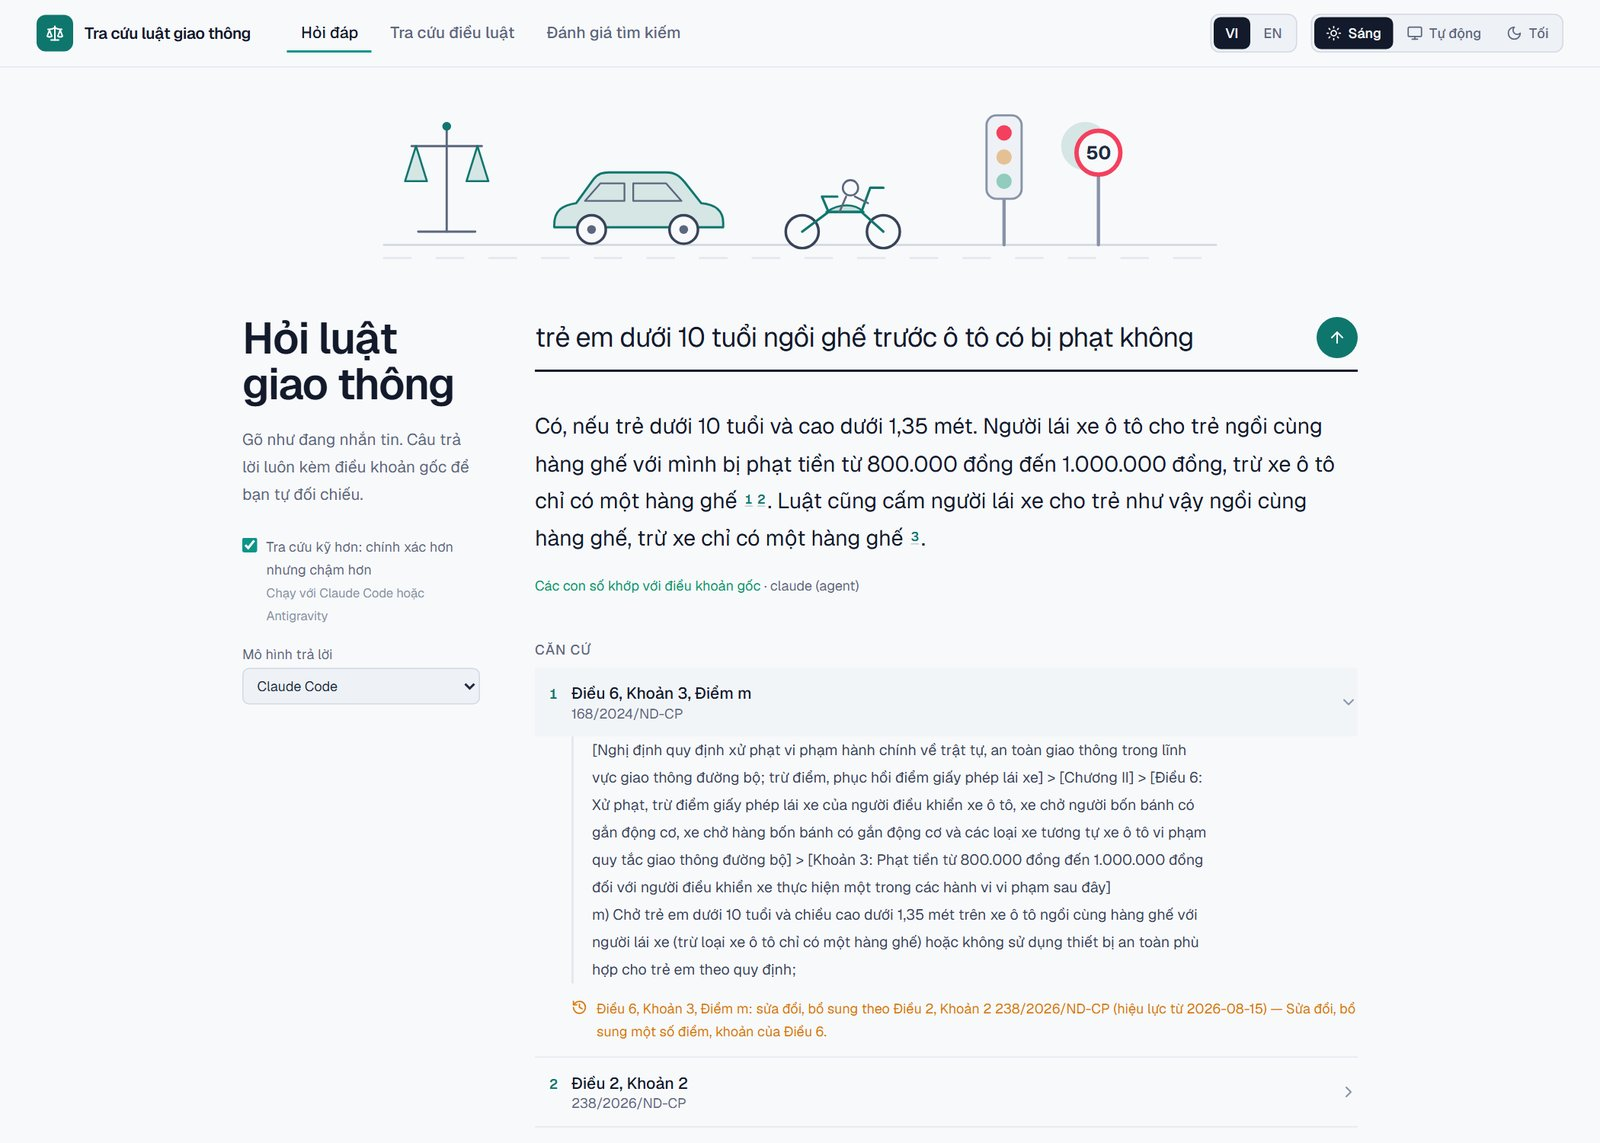
\includegraphics[width=0.88\textwidth]{graphics/ui_hoidap_traloi.jpg}
\caption[Kết quả hỏi đáp ở chế độ agent]{Kết quả hỏi đáp ở chế độ agent cho câu hỏi về trẻ em dưới 10 tuổi ngồi ghế trước ô tô: câu trả lời có trích dẫn, nguyên văn điều khoản nguồn và ghi chú sửa đổi theo Nghị định 238/2026/NĐ-CP}
\label{fig:ui-traloi}
\end{figure}

\begin{figure}[H]
\centering
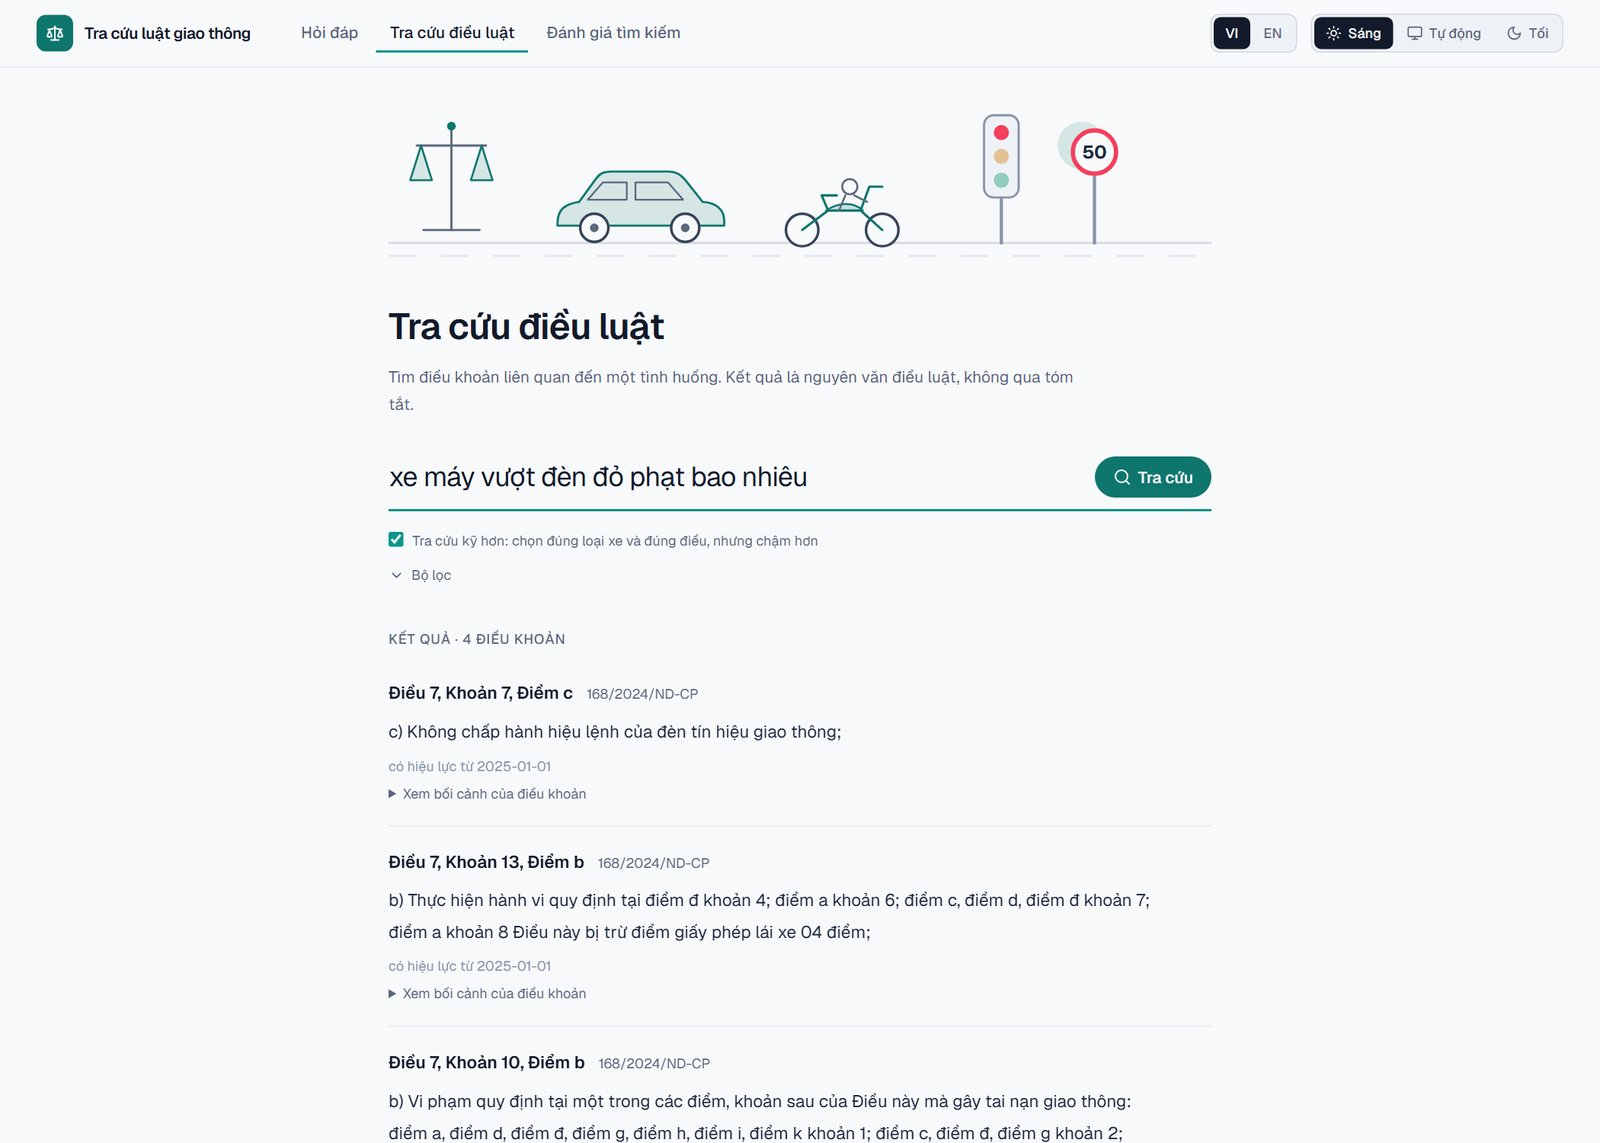
\includegraphics[width=0.78\textwidth]{graphics/ui_tracuu_ky.jpg}
\caption[Chế độ ``Tra cứu kỹ hơn'']{Chế độ ``Tra cứu kỹ hơn'' cho tình huống vượt đèn đỏ bằng xe máy: agent đưa Điểm c Khoản 7 Điều 7 Nghị định 168/2024/NĐ-CP lên đầu danh sách}
\label{fig:ui-tracuu-ky}
\end{figure}

\begin{figure}[H]
\centering
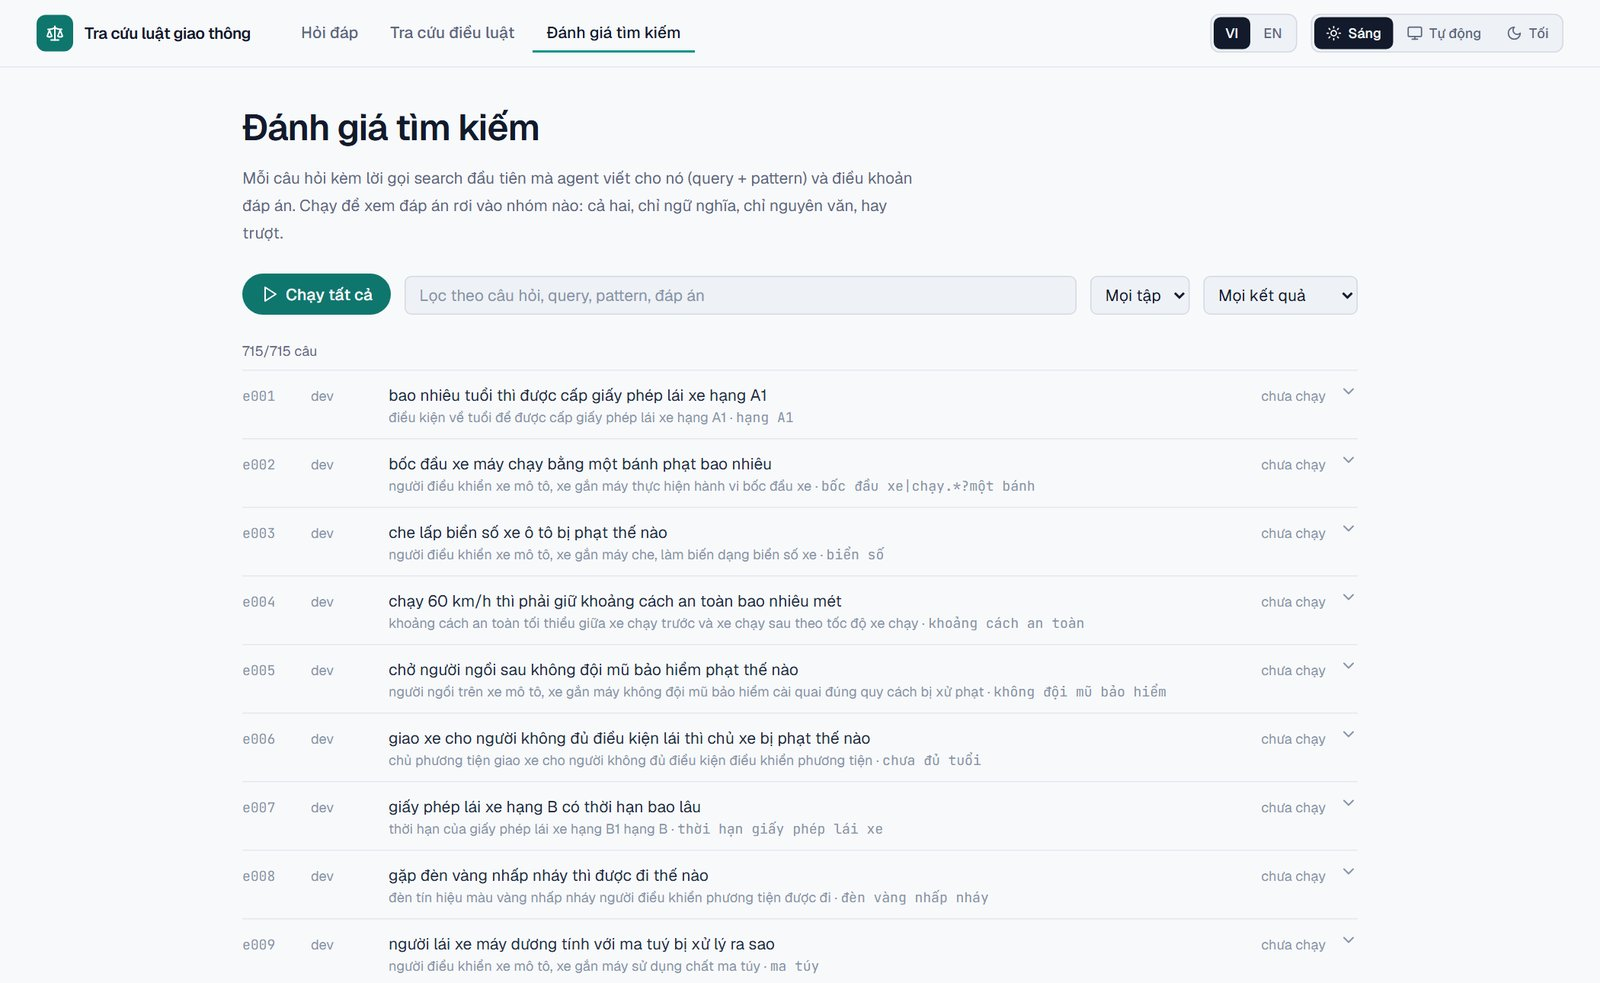
\includegraphics[width=0.78\textwidth]{graphics/ui_danhgia.jpg}
\caption{Thẻ Đánh giá: xem, sửa và chạy các câu của bộ đánh giá tìm kiếm}
\label{fig:ui-danhgia}
\end{figure}

\begin{figure}[H]
\centering
\begin{subfigure}[b]{0.62\textwidth}
  \centering
  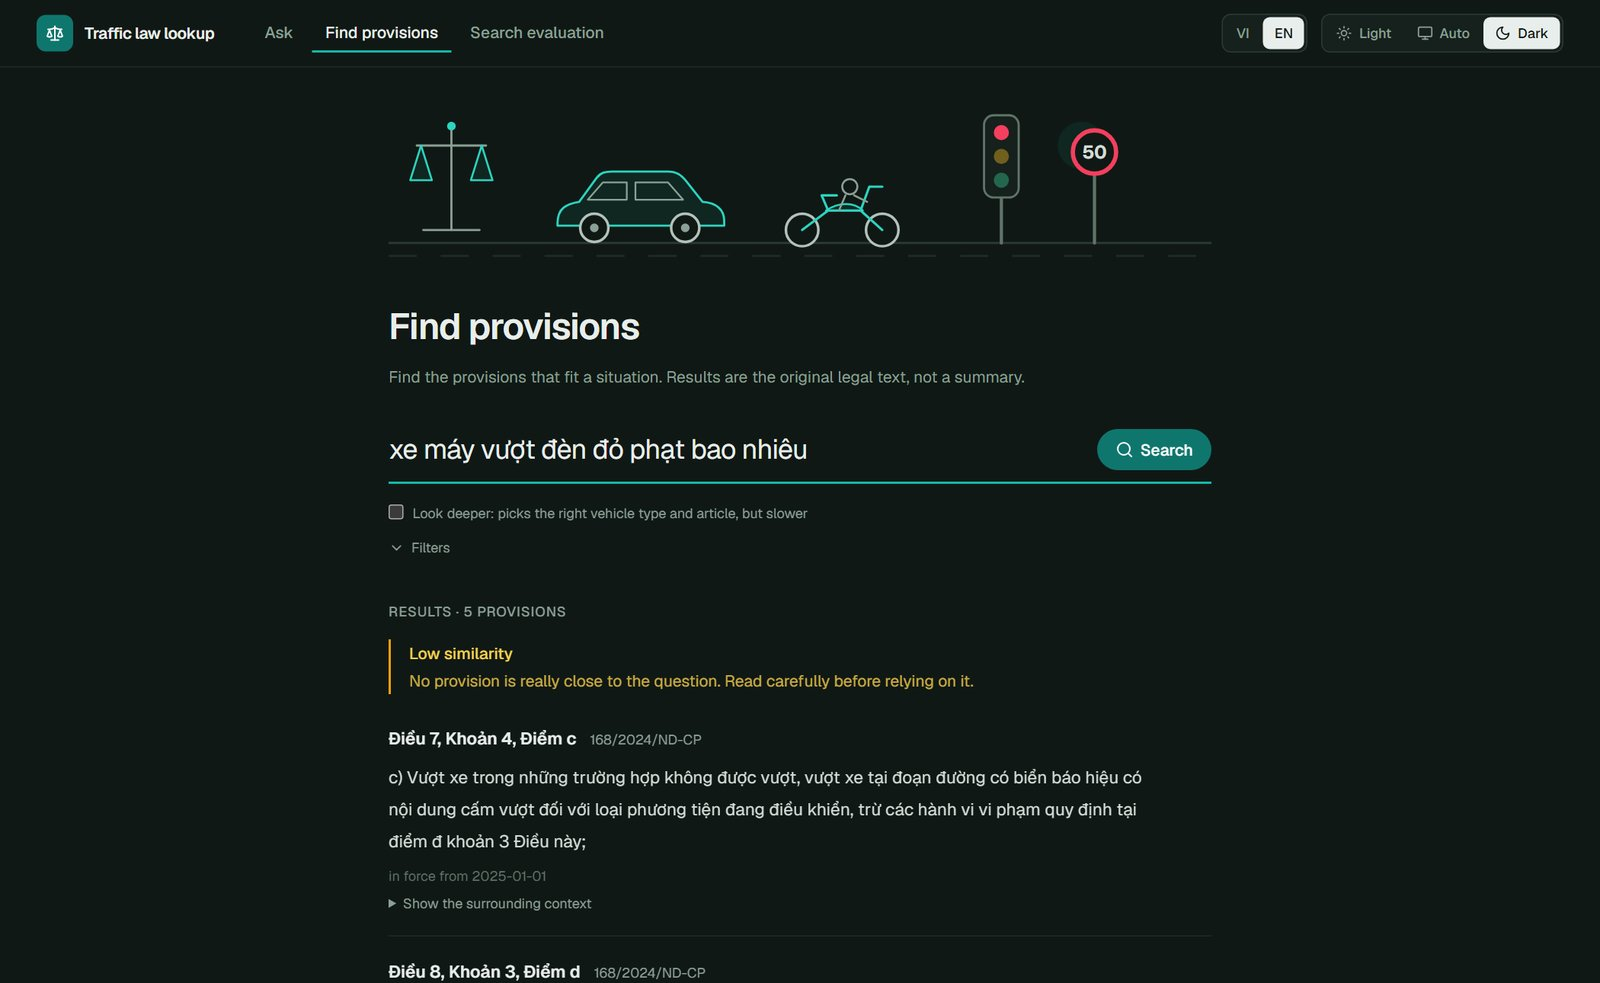
\includegraphics[width=\textwidth]{graphics/ui_tracuu_en_toi.jpg}
  \caption{Giao diện tiếng Anh, chế độ tối}
\end{subfigure}
\hfill
\begin{subfigure}[b]{0.30\textwidth}
  \centering
  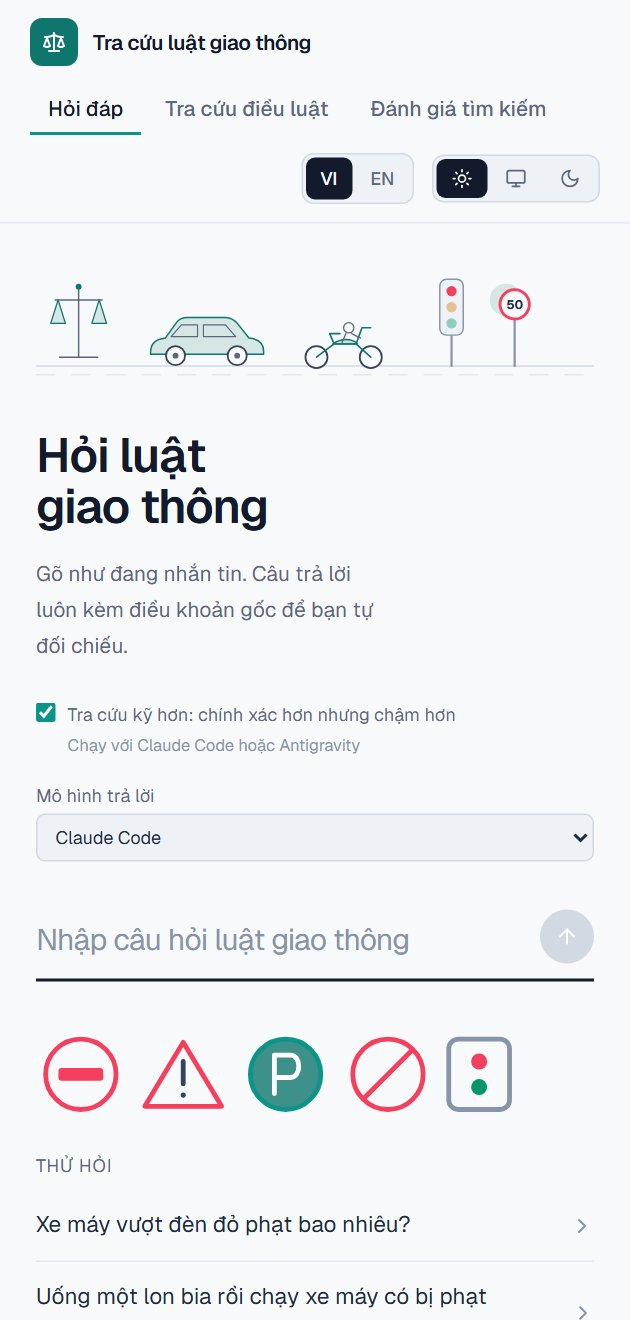
\includegraphics[width=\textwidth]{graphics/ui_mobile.jpg}
  \caption{Bố cục trên điện thoại}
\end{subfigure}
\caption{Hỗ trợ song ngữ, chế độ màu và màn hình nhỏ}
\label{fig:ui-dapung}
\end{figure}
